\documentclass[10pt]{article}
\usepackage[export]{adjustbox}
\usepackage{amsmath}
\usepackage[makeroom]{cancel}
\usepackage{enumitem}
\usepackage{graphicx}
%Load mhchem using some package options
\usepackage[version=4]{mhchem}
\usepackage{multicol}
\usepackage{siunitx}

\title{
    Problem Set \#5
    \\  \small
    CHEM101A: General College Chemistry
    }
\author{Donald Aingworth IV}
\date{September 19, 2025}

\begin{document}
    \DeclareSIUnit{\atm}{atm}
    \DeclareSIUnit{\molarity}{M}
    \DeclareSIUnit{\M}{M}

    \maketitle

    \setcounter{section}{9}

    \pagebreak
    \section{Topic C Problem 10}
        This question is intended to give you a “feel” for the size of the SI energy unit.
        a) Jorge weighs 69.0 kg (152 pounds). If he is walking at a speed of 1.12 m/sec (about 2.5 miles per hour), what is his kinetic energy in joules? 
        b) If Jorge's kinetic energy is 1.00 J, how fast is he moving?

        \subsection{Solution}

    \pagebreak
    \section{Topic C Problem 11}
        The average kinetic energy of the atoms in a sample of gaseous argon at a certain temperature is 5188 J/mol.
        \begin{enumerate} [label=\alph*)]
            \item What is the average kinetic energy of a single argon atom, in joules?
            \item If a argon atom has the kinetic energy you calculated in part a, how fast is it moving?
            \item If the argon sample weighs 1.450 g, what is the total kinetic energy of the atoms in the sample?
            \item What is the temperature of the argon?
            \item What is the most probable kinetic energy for the argon, in J/mol?
            \item What is the root-mean-square speed of the argon atoms?
            \item What is the average speed of the argon?
            \item What is the most probable speed of the argon atoms?
        \end{enumerate}

        \subsection{Solution}

    \pagebreak
    \section{Topic C Problem 12}
        A molecule of nitrogen trifluoride is moving at 426 m/sec at 25\unit{\celsius}.
        \begin{enumerate} [label=\alph*)]
            \item What is the kinetic energy of this molecule, in joules?
            \item What is the kinetic energy of this molecule, in J/mol?
            \item Is this molecule moving faster than the average speed of nitrogen trifluoride molecules at this temperature?
        \end{enumerate}

        \subsection{Solution}

    \pagebreak
    \section{Topic C Problem 13}
        A sample of \ce{O2} is at 100\unit{\celsius}.
        \begin{enumerate} [label=\alph*)]
            \item What temperature would a sample of \ce{O3} (ozone) need to be in order for it to have the same average kinetic energy as the \ce{O2}?
            \item What temperature would the \ce{O3} need to be in order for it to have the same average molecular speed as the \ce{O2}?
            \item What temperature would the \ce{O3} need to be in order for it to have the same root-mean-square speed as the \ce{O2}?
        \end{enumerate}

        \subsection{Solution}

    \pagebreak
    \section{Topic C Problem 14}
        Two identical containers are filled with gases as shown below:
        
        Container 1: \ce{N2O(g)} at 0\unit{\celsius}, 700 torr
        
        Container 2: \ce{NO2(g)} at 0\unit{\celsius}, 700 torr
        \begin{enumerate} [label=\alph*)]
            \item Which gas has the higher rms speed? Explain how you can tell.
            \item Which gas has the higher KEmp (most probable kinetic energy)? Explain.
            \item Which gas weighs more? Explain how you can tell.
        \end{enumerate}

        \subsection{Solution}

    \pagebreak
    \section{Topic C Problem 15}
        Two identical containers are filled with gases as shown below:
        
        Container 1: NO2 at 200ºC, 1 atm 
        
        Container 2: NO at 100ºC, 1 atm
        
        \begin{enumerate} [label=\alph*)]
            \item Which gas has the higher average kinetic energy? Explain how you can tell.
            \item Which gas has the higher most probable speed? Explain how you can tell.
            \item Which gas weighs more? Explain how you can tell.
        \end{enumerate}

        \subsection{Solution}

    \pagebreak
    \section{Topic C Problem 16}
        Explain the following observations, using the kinetic theory of gases.
        \begin{enumerate} [label=\alph*)]
            \item When a gas is heated, the pressure that it exerts increases.
            \item Gases can easily be compressed into smaller volumes.
            \item Raising the temperature of 1 mole of helium by 1\unit{\celsius} requires the same amount of energy as raising the temperature of 1 mole of argon by 1\unit{\celsius}.
        \end{enumerate}

        \subsection{Solution}

    \pagebreak
    \section{Topic C Problem 17}
        Two identical containers are filled with gases as shown below: 
        
        Container 1: \ce{CH4} at 0\unit{\celsius}, 1 atm 
        
        Container 2: \ce{C2H6} at 0\unit{\celsius}, 1 atm

        \begin{enumerate} [label=\alph*)]
            \item Which gas has a larger fraction of molecules with kinetic energies greater than 5000 J/mol? Explain how you can tell.
            \item Which gas has a larger fraction of molecules with speeds less than 500 m/sec? Explain how you can tell.
        \end{enumerate}

        \subsection{Solution (a)}
            KE is only proportional to the temperature.
            If the temperature is identical for both, roughly an equal fraction of each would have a kinetic energy greater than 5000\,\unit{\joule/\mole}. 
            The answer is \boxed{\rm neither}. 

        \subsection{Solution (b)}
            Velocity is inversely proportional to the molar mass.
            \ce{C2H6} inevitably has a higher molar mass.
            This means it will have lower general velocity and more velocity below a certain value.
            The answer is \boxed{\ce{C2H6}}. 

    \pagebreak
    \section{Topic C Problem 18}
        Two identical containers are filled with gases as shown below:

        Container 1: \ce{Ar} at 100\unit{\celsius}, 1 atm 
        
        Container 2: \ce{CO2} at 125\unit{\celsius}, 1 atm

        \begin{enumerate} [label=\alph*)]
            \item Which gas has a larger fraction of molecules with kinetic energies lower than 5000 J/mol? Explain how you can tell.
            \item Which gas has a larger fraction of molecules with speeds above 500 m/sec? Explain how you can tell.
        \end{enumerate}

        \subsection{Solution (a)}
            When considering these differences, I tend to consider the formulas for either the average or most probable kinetic energies and/or velocities.
            I'll stick with kinetic energy here, specifically the most probable.
            \begin{equation}
                \rm
                KE_{\rm mp} = \frac{1}{2}RT
            \end{equation}

            This says that kinetic energy is directly proportional to temperature. 
            This means that the one with lower temperature will have more data lower.
            Since we are looking for the gas with a larger fraction of molecules \textit{lower} than the target value, the one with the lower MP value (and the lower temperature) would have more molecules less than that value.
            That would be \boxed{\text{Ar}}. 

        \subsection{Solution (b)}
            Just find the one with the higher most probable or average velocity.
            Both are proportional (not directly but not inversely) to the fraction of $\frac{T}{MM}$. 
            We can calculate that for both.
            \begin{align}
                MM(\ce{Ar}) &=  39.95\,\unit{\gram/\mole}\\
                MM(\ce{CO2})&=  12.01 + 2 * 16.00
                    =   44.01\,\unit{\gram/\mole}\\
                T_{\ce{Ar}} &=  100\unit{\celsius} + 273.15\unit{\kelvin}
                    =   373.15\unit{\kelvin}\\
                T_{\ce{CO2}}&=  125\unit{\celsius} + 273.15\unit{\kelvin}
                    =   398.15\unit{\kelvin}\\
                \frac{T_{\ce{Ar}}}{MM(\ce{Ar})} &=  \frac{373.15\unit{\kelvin}}{39.95\,\unit{\gram/\mole}}
                    \approx 9.34\,\unit{\frac{\kelvin\cdot\mole}{\gram}}\\
                \frac{T_{\ce{CO2}}}{MM(\ce{CO2})}   &=  \frac{398.15\unit{\kelvin}}{44.01\,\unit{\gram/\mole}}
                    \approx 9.05\,\unit{\frac{\kelvin\cdot\mole}{\gram}}
            \end{align}

            Since the value for \ce{Ar} is greater, its velocity would be greter and the answer would be \boxed{\text{Ar}}. 

    \pagebreak
    \section{Topic C Problem 19}
        The graph below shows the kinetic energy distribution for \ce{N2(g)} at an unknown temperature.
        \begin{center}
            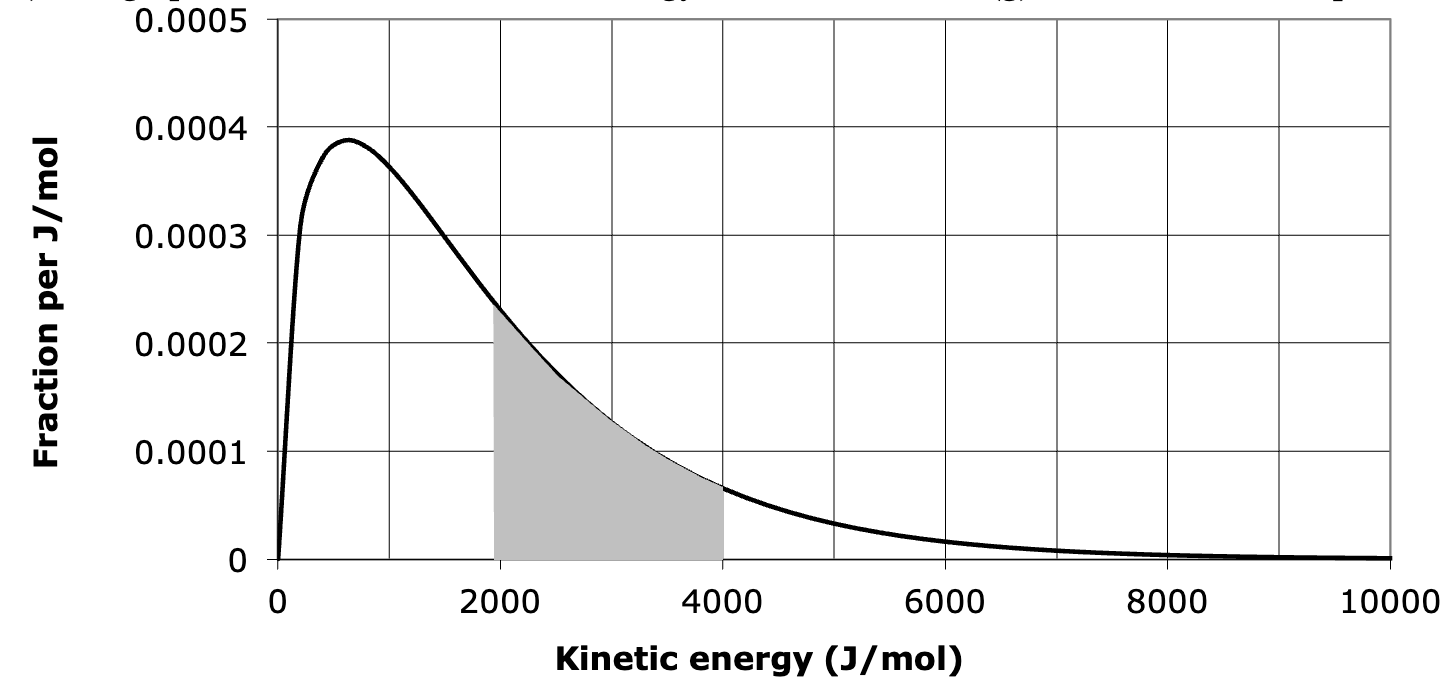
\includegraphics[width=\textwidth]{picture_C-19.png}
        \end{center}
        
        \begin{enumerate} [label=\alph*)]
            \item What is the most probable kinetic energy for the gas, based on the graph?
            \item What is the approximate temperature of the gas, based on your answer to part a?
            \item What is the $y$ value when $x$ = 2000 J/mol? What does this $y$ value tell you?
            \item The area of the shaded region is 0.259. What does this value tell you?
        \end{enumerate}

        \subsection{Solution (a)}
            This is found at the peak of the graph.
            That point has the x-value of roughly \boxed{700\,\unit{\joule/\mole}}. 

        \subsection{Solution (b)}
            We can use the most probable kinetic energy for this. 
            \begin{gather}
                K_{\rm mp} = \frac{1}{2} RT \to
                T   =   \frac{2K_{\rm mp}}{R}
                    =   \frac{2 * 700}{8.314}
                    =   \frac{1400}{8.314}
                    =   \boxed{168.4\,\unit{\kelvin}}
            \end{gather}
        
        \subsection{Solution (c)}
            The $y$ value is roughly \boxed{0.00023}. 
            This means that roughly 0.023\% of all molecules have a kinetic energy of 2000\,\unit{\joule/\mole}. 
        
        \subsection{Solution (d)}
            This meas that 25.9\% of all molecules have a kinetic energy between roughly 2000\,\unit{\joule/\mole} and 4000\,\unit{\joule/\mole}. 

    \pagebreak
    \section{Topic C Problem 20}
        The following questions relate to the graph below, in which curve B represents the kinetic energy distribution for \ce{Ne(g)} at 300 K.

        a) Which curve (A, B, or C) could represent the kinetic energy distribution for \ce{Ar(g)} at 300 K? Explain your answer briefly.

        b) Which curve could represent the kinetic energy distribution for \ce{Ne(g)} at 150 K? Explain your answer briefly.

        \begin{center}
            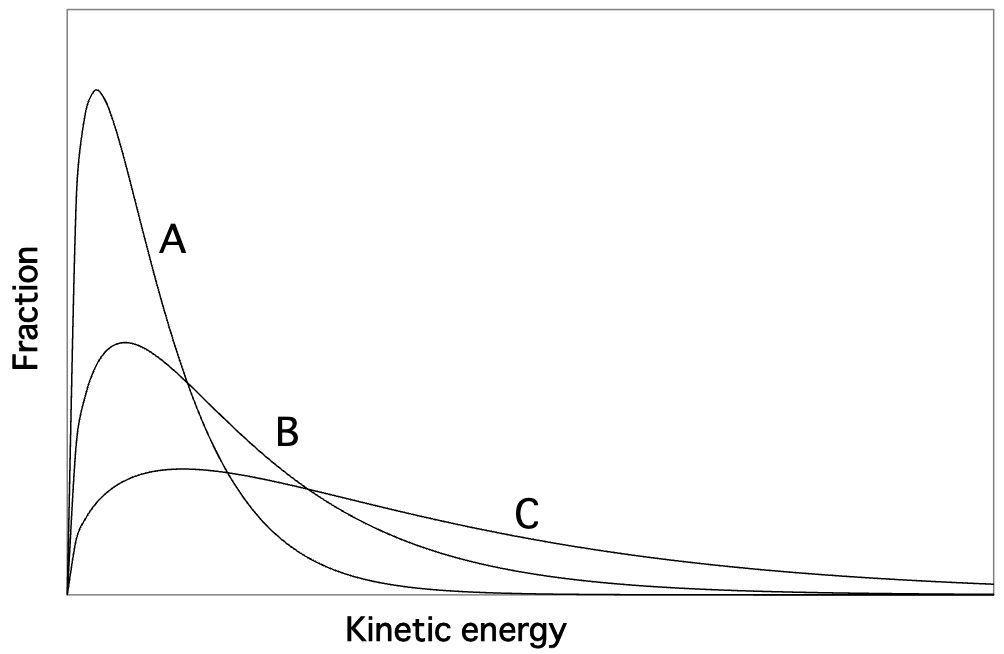
\includegraphics[width=\textwidth]{picture_C-20.png}
        \end{center}

        \subsection{Solution (a)}
            Molar mass has no effect on kinetic energy. 
            This means the curves would be identical, so the curve would be \boxed{B}.

        \subsection{Solution (b)}
            The most probeble Kinetic Energy is directly related to the temperature.
            As the temperature would decrease, the most probable Kinetic Energy (the peak) would also decrease.
            Since the peak would be at a lower Kinetic Energy, the one that would have a peak at a lower Kinetic Energy would be \boxed{A}.

    \pagebreak
    \section{Topic C Problem 21}
        Consider the graph below, in which curve B represents the distribution of speeds for \ce{N2(g)} at 25.0\unit{\celsius}.
        \begin{center}
            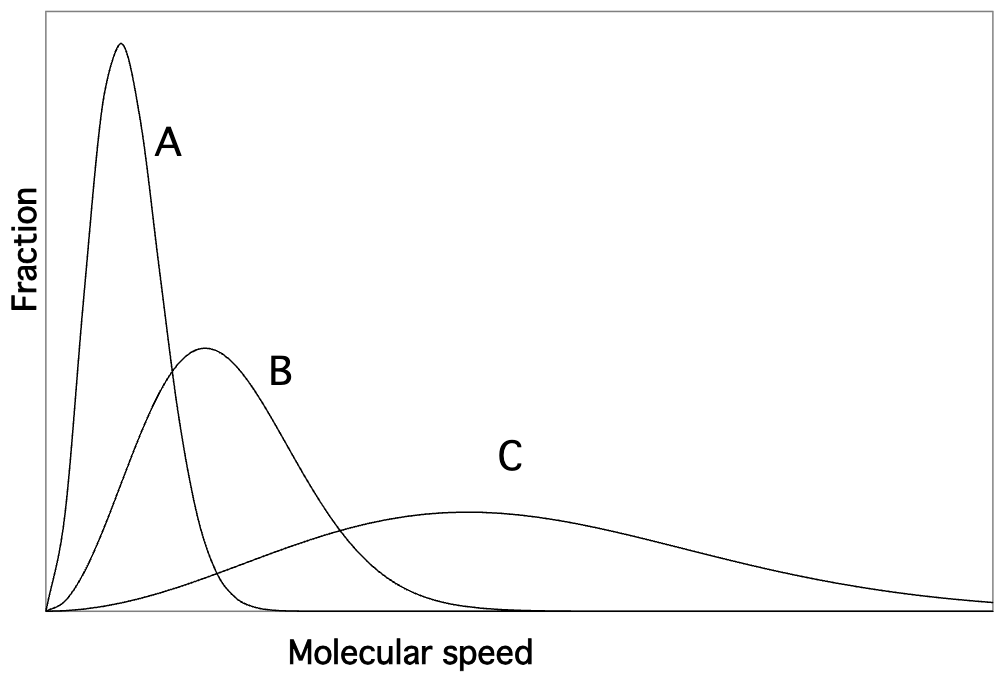
\includegraphics[width=\textwidth]{picture_C-21.png}
        \end{center}

        \begin{enumerate} [label=\alph*)]
            \item Which curve (A, B, or C) could represent the distribution of speeds for \ce{N2(g)} at $-125.0\unit{\celsius}$? Explain your answer briefly.
            \item Which curve could represent the distribution of speeds for \ce{H2(g)} at \\25.0\unit{\celsius}? Explain your answer briefly.
            \item Which curve could represent the distribution of speeds for \ce{Ne(g)} at \\$-58.4\unit{\celsius}$? Explain your answer briefly.
        \end{enumerate}

        \subsection{Solution (a)}
            The formula of the most probably velocity ($v_{\rm mp}$) is simple.
            \begin{equation}
                v_{\rm mp}  =   \sqrt{\frac{2RT}{M}}
            \end{equation}

            As the temperature would decrease, the most probable velocity (the peak) would also decrease.
            Since the peak would be at a lower velocity, the one that would have a peak at a lower molecular speed would be \boxed{A}.

        \subsection{Solution (b)}
            \ce{H2(g)} has a lower molar mass than \ce{N2(g)}. 
            Looking at the formula for the peak (most probably velocity), as the molar mass decreases, the most probable velocity (the peak) would increase. 
            The curve that fits this description would be \boxed{C}.

        \subsection{Solution (c)}
            Measure the value of $\frac{T_1 / M_1}{T_2 / M_2}$. 
            \begin{align}
                \frac{T_1 / M_1}{T_2 / M_2} &=  \frac{T_1}{T_2} * \frac{M_2}{M_1}
                    =   \frac{25 + 273.15}{-58.4 + 273.15} * \frac{20.18}{28.02}\\
                    &=  \frac{298.15}{215.75} * \frac{20.18}{28.02}
                    \approx 1
            \end{align}
            
            This means that the change from the temperature and moral mass more or less evens out to little change.
            Conclusively, this means that the best graph would be \boxed{B}. 

    \pagebreak
    \section{Topic C Problem 22}
        The graph below shows the distribution of speeds for an unknown gas at 200\unit{\celsius}.
        \begin{enumerate} [label=\alph*)]
            \item What is the most probable speed for this gas?
            \item This gas is one of the inert gases. Which one is it, and how did you determine this?
            \item What is the y value when x = 200 m/sec? What does this y value tell you?
            \item The area of the shaded region (which extends out to infinite speed) is 0.111. What does this value tell you?
            \item What is the area of the region under the curve that is not shaded? What does this value tell you?
        \end{enumerate}
        \begin{center}
            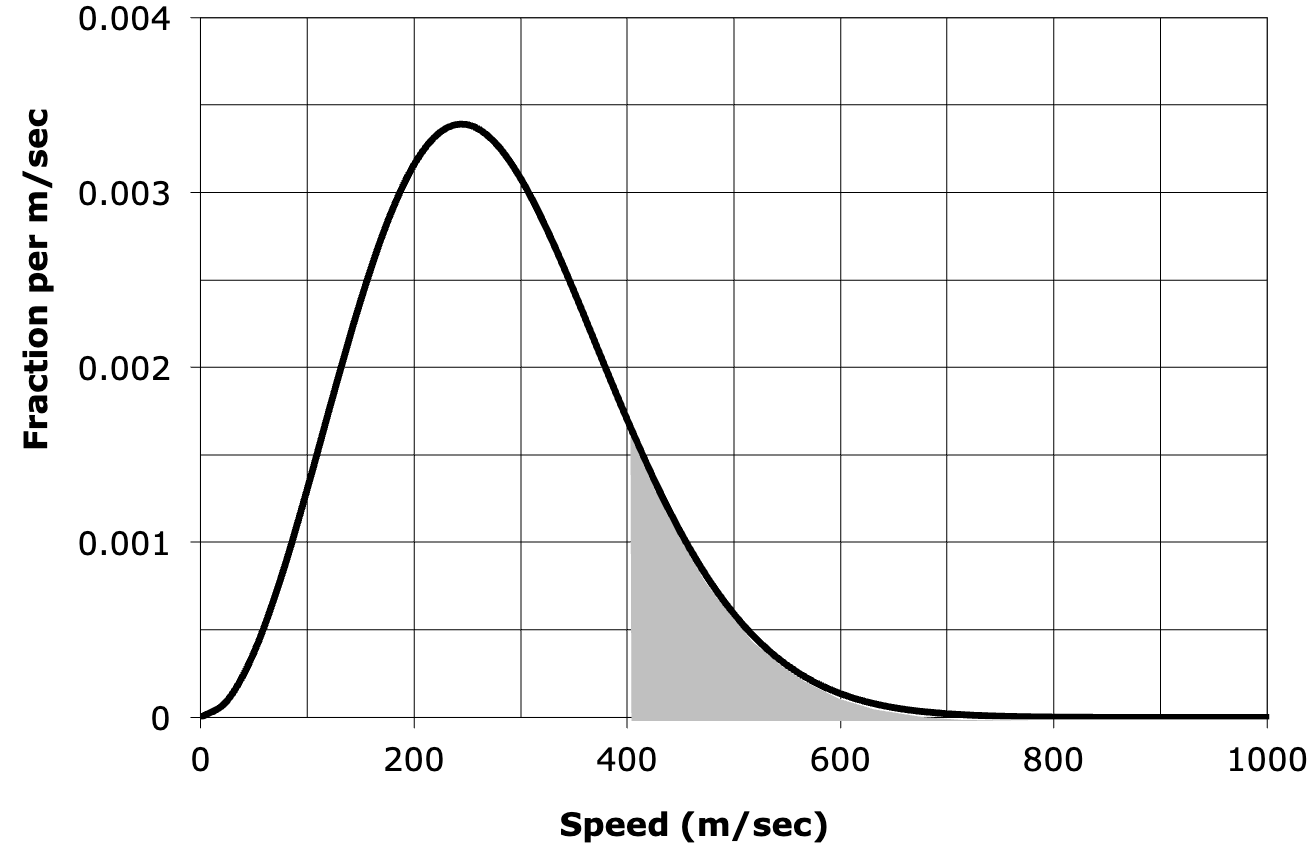
\includegraphics[width=\textwidth]{picture_C-22.png}
        \end{center}

        \subsection{Solution (a)}
            The most probably speed is about \boxed{240\,\unit{\meter/\second}}, the peak. 
            The large size of the divisions makes it difficult to see the peak of the graph.

        \subsection{Solution (b)}
            The most probable speed is about 240\,\unit{\meter/\second}. 
            At 200\unit{\celsius}, the temperature in kelvin is 473.15\unit{\kelvin} and this can be used to find the molar mass.
            \begin{gather}
                v_{\rm mp}  =   \sqrt{\frac{2RT}{MM}}   \to
                v_{\rm mp}^2=   \frac{2RT}{MM}\\
                \begin{align}
                    MM  &=  \frac{2RT}{v_{\rm mp}^2}
                        =   \frac{2*8.31*473.15}{240^2}
                        =   \frac{7863.753}{57600}\,\unit{\kilo\gram/\mole}\\
                        &=  0.1365\,\unit{\kilo\gram/\mole}
                        =   136.5\unit{\gram/\mole}
                        \approx MM\left( \boxed{\ce{Xe(g)}} \right)
                \end{align}
            \end{gather}

        \subsection{Solution (c)}
            At $x = 200\,\unit{\meter/\second}$, $f(x) \approx \boxed{0.0032}$.
            This tells us that approximately 0.32\% of all molecules in the sample would have a speed of exactly 200\,\unit{\meter/\second}. 
            Looking at the answer key, I would disagree that it would be 0.0033. 
            If you look at the graph, the smallest divisions are are 0.0005.
            The intersection of the function with the line is below the halfway point between the 0.0030 and 0.0035 lines.
            This makes it impossible to be greater than 0.00325, which 0.0033 is greater than and as such an impossible value.
            Then again, maybe my eyes are bad.

        \subsection{Solution (d)}
            It tells us that 11.1\% of all particles are faster than 400\,\unit{\meter/\second}.

        \subsection{Solution (e)}
            Since the total area under the curve is 1 and all the area is either shaded or not shaded, the area not shaded would be $1 - 0.111 = \boxed{0.889}$.
            This tells us that about 88.9\% of all particles are slower than 400\,\unit{\meter/\second}.

    \pagebreak
    \section{Topic C Problem 23}
        At 62\unit{\celsius}, 5.00 mL of argon effuses through a porous barrier in 5 minutes and 13 seconds. 
        In an identical apparatus at 62\unit{\celsius}, 5.00 mL of an unknown gas effuses through the barrier in 4 minutes and 22 seconds. 
        The empirical formula of the unknown gas is \ce{CH2}. 
        Determine the molecular formula of the gas.

        \subsection{Solution}
            We can use the formula of the relation between molar masses and effusion rates.
            First, we calculate the time in seconds for each.
            Argon would be momoatomic in this case. 
            I will be calling the gas \ce{xCH2}.
            \begin{align}
                t_{\ce{Ar}} &=  5 * 60 + 13
                    =   313\,\unit{\second}\\
                t_{\ce{xCH2}}&=  4 * 60 + 22
                    =   262\,\unit{\second}
            \end{align}

            Now we use the formula.
            \begin{gather}
                \frac{\text{rate \ce{Ar}}}{\text{rate \ce{xCH2}}}    =   \frac{5\,\unit{\milli\liter}/313\,\unit{\second}}{5\,\unit{\milli\liter}/262\,\unit{\second}}
                    =   \frac{262}{313}
                    =   \frac{\sqrt{MM(\ce{xCH2})}}{\sqrt{MM(\ce{Ar})}}\\
                MM(\ce{Ar}) =   39.95\,\unit{\gram/\mole}\\
                \begin{align}
                    \sqrt{MM(\ce{xCH2})} &=  \sqrt{MM(\ce{Ar})} * \frac{262}{313}
                        =   \sqrt{39.95\unit{\gram/\mole}} * \frac{262}{313}\\
                    MM(\ce{xCH2})    &=  39.95\,\unit{\gram/\mole} * \frac{262^2}{313^2}
                        =   39.95\,\unit{\gram/\mole} * 0.701\\
                        &=  27.992\,\unit{\gram/\mole}
                \end{align}
            \end{gather}

            We can calculate the molar mass of empirical \ce{CH2}. 
            That in turn can be used to find the number of carbon and/or dihydrogen in eventual formula.
            \begin{align}
                MM(\ce{CH2})    &=  12.01\,\unit{\gram/\mole} + 2 * 1.008\,\unit{\gram/\mole}
                    =   14.028\,\unit{\gram/\mole}\\
                x   &=  \frac{MM(\ce{xCH2})}{MM(\ce{CH2})}
                    =   \frac{27.992\,\unit{\gram/\mole}}{14.028\,\unit{\gram/\mole}}
                    \approx 2
            \end{align}

            This sets the final formula of the chemical to be \boxed{\ce{C2H4}}. 

    \pagebreak
    \section{Topic C Problem 24}
        If we compare the van der Waals constants for water and nitrogen, we see that water has a higher value of $a$ while nitrogen has a higher value of $b$. 
        The numbers are:

        \ce{H2O}: $a$ = 5.46 atm·L$^2$/mol$^2$ $b$ = 0.0305 L/mol

        \ce{N2}: $a$ = 1.39 atm·L$^2$/mol$^2$ $b$ = 0.0391 L/mol

        a) Explain why water has the higher $a$ value.

        b) Explain why nitrogen has the higher $b$ value.

        \subsection{Solution (a)}
            $a$ is a measure for the pressure, in and of a measurement of the attraction of particles. 
            I cannot explain \ce{H2O} having a higher value of $a$ due ot Physical and atomic factors. 
            I can explain why it makes sense with regard to the physical properties of \ce{H2O}.
            \ce{H2O} has a higher boiling point than \ce{N2}. 
            Boiling and freezing points are measurements of the points at which the gas cannot overcome the intermolecular forces that control the pressure and condense into a separate state of matter (in this case liquid).
            Since \ce{H2O} has a much higher boiling point than \ce{N2}, that would mean that the intermolecular forces are also significantly higher, as would be the pressure.
            Since pressure from the Ideal Gas Law is not affected by the molar mass, it would have to be affected by something unrelated to the Ideal Gas Law, namely $a$. 
            This is why $a$ would be higher for \ce{H2O}. 

        \subsection{Solution (b)}
            $b$ is a measure regarding the volume. 
            As the volume of each molecule increases, the value of $b$ shold also increase.
            \ce{N2}, being made up of two nitrogen atoms, is made up of a total of 14 protons, about as many neutrons, and a couple fewer electrons. 
            \ce{H2O}, meanwhile, would be made up of two Hydrogen atoms and one Oxygen atom, totaling ten protons, about as many neutrons, and eight electrons. 
            Assuming all protons to have equal volume and due to this, as well Oxygen keeping its electrons closer to itself than Nitrogen, the \ce{N2} have a larger overall volume than the \ce{H2O}. 
            This would lead to the \ce{N2} having a higher value of $b$. 

    \pagebreak
    \section{Topic C Problem 25}
        An engineer is designing a reactor that will be filled with oxygen under high pressure. 
        The volume of the reactor is 253 L, the maximum temperature inside the reactor will be 250\unit{\celsius}, and the pressure inside the reactor must not exceed 150 atm. 
        The engineer uses the ideal gas law to calculate the maximum number of moles of oxygen that can be put into the reactor without exceeding 150 atm.

        \begin{enumerate} [label=\alph*)]
            \item What number of moles does the engineer calculate using the ideal gas law?
            \item Now use the van der Waals equation to calculate a more accurate value for the pressure inside the reactor at 250\unit{\celsius}, using the number of moles you obtained in part $a$. (Van der Waals constants for oxygen are given in the textbook.)
            \item Based on your answers to parts $a$ and $b$, was the engineer justified in using the ideal gas law, or will she create an unsafe situation? Explain your answer briefly.
        \end{enumerate}

        \subsection{Solution (a)}
            Use the Ideal Gas Law. 
            \begin{gather}
                PV  =   nRT\\
                \begin{align}
                    n   &=  \frac{PV}{RT}
                        =   \frac{150\,\unit{\atm} \times 253\,\unit{\liter}}{(250\unit{\celsius} + 273.15\unit{\kelvin}) \times 0.08206\,\unit{\atm\cdot\liter/\mol\cdot\kelvin}}\\
                        &=  \frac{37950}{42.929689}\,\unit{\mole}
                        =   884.004\,\unit{\mole}
                        \approx \boxed{884\,\unit{\mole}}
                \end{align}
            \end{gather}

        \subsection{Solution (b)}
            Use the Van der Waals equation. 
            The values to be used are $a = 1.364\,\unit{\frac{L^2\cdot\atm}{\mole^2}}$ and $b = 0.0319\,\unit{\liter/\mole}$. 
            \begin{gather}
                P \to P + a \left( \frac{n}{V} \right)^2\\
                \begin{align}
                    P + a \left( \frac{n}{V} \right)^2  &=  250\,\unit{\atm} + 1.364\,\unit{\frac{L^2\cdot\atm}{\mole^2}} * \left( \frac{884.004\,\unit{\mole}}{253\unit{\mole}} \right)^2\\
                        &=  250\,\unit{atm} + 16.65\,\unit{\atm}
                        =   \boxed{266.7\,\unit{\atm}}
                \end{align}
            \end{gather}

        \subsection{Solution (c)}
            If there was some room for error (e.g. by 17 atm), then it would be reasonable. 
            However, there appears not to be room for error for the pressure, so the pressure would have to be the 150 atm or less.
            Were the user to use the supposed suggested amount of moles, the reactor would be very unsafe.
            The answer is \boxed{no}. 

    \pagebreak
    \section{Topic C Problem 26}
        The graph below shows how the actual pressure of a sample of \ce{O2} deviates from the ideal gas prediction. 
        The values on the y axis are the actual pressure of the gas divided by the pressure calculated from the ideal gas law. 
        (A y value of 1 means the actual pressure equals the ideal gas prediction.)
        \begin{center}
            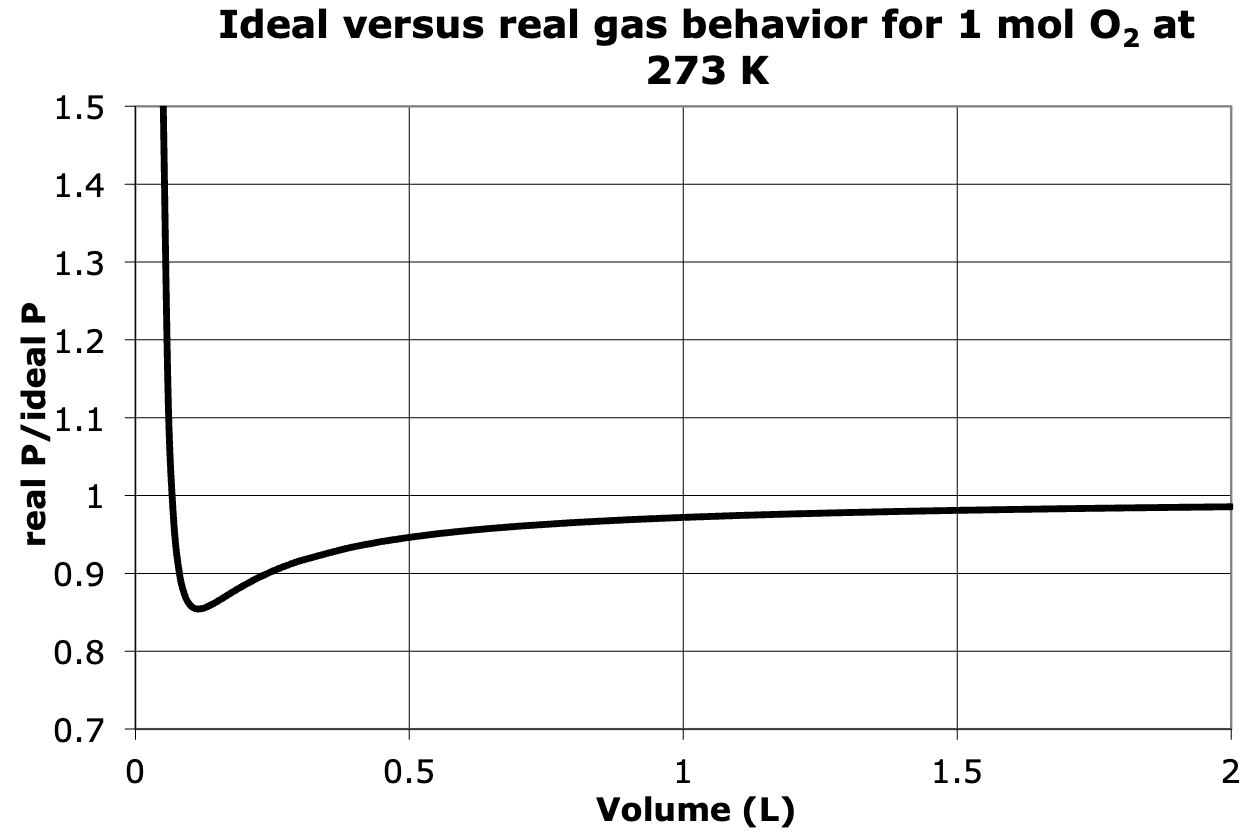
\includegraphics[width=\textwidth]{picture_C-26.png}
        \end{center}

        a) Based on this graph, under what conditions is the actual pressure lower than the ideal gas prediction? 
        Why is this?
        
        b) Based on this graph, under what conditions is the actual pressure higher than the ideal gas prediction? 
        Why is this?

        \subsection{Solution (a)}
            Whenever the value of $\frac{real\,P}{ideal\,P}$ is less than 1, the actual pressure is less than the ideal pressure.
            Looking at the graph, it is always less than 1 after the time it is initially equal to 1. 
            That point is approximately one sizth of the way between 0 and 0.5. 
            Multiplying those together, we get $\frac{1}{6} \times 0.5 = \frac{1}{12}$. 
            As such, the range where we know that the actual pressure is lower than the ideal gas prediction is \boxed{\left(\frac{1}{12},2\right]}. 

        \subsection{Solution (b)}
            This is pretty much the opposite case, but my answer has largely the same meaning. 
            Unless the value of $\frac{real\,P}{ideal\,P}$ is not continuous and permanantly jumps to less than 0.7 somewhere between $V = 0$ and $V = \frac{1}{12}$, the range of this condition is \boxed{\left[0, \frac{1}{12}\right)}

    \pagebreak

    \tableofcontents
\end{document}